\section{Simulation}

\subsection{Erläuterung zu der Simulation}
Die Antenne wurde über mehrere Simulationsschritte verfeinert, so dass sie das gewünschte Verhalten aufzeigt. Gemäss Simulation sollte die Antenne einen Reflexionsfaktor von knapp -16dB aufweisen bei einer Frequenz von 2.4GHz. Die reale Impedanz liegt gemäss Simulation bei 2.4 GHz bei 43 Ohm, der Imaginäranteil bei 14 Ohm induktiv. Der Imaginäranteil wurde bewusst im positiven Bereich gelassen, damit zur Kompensation ein C angebracht werden könnte.

\subsubsection{Modell}

\begin{figure}[h!]
	\centering
	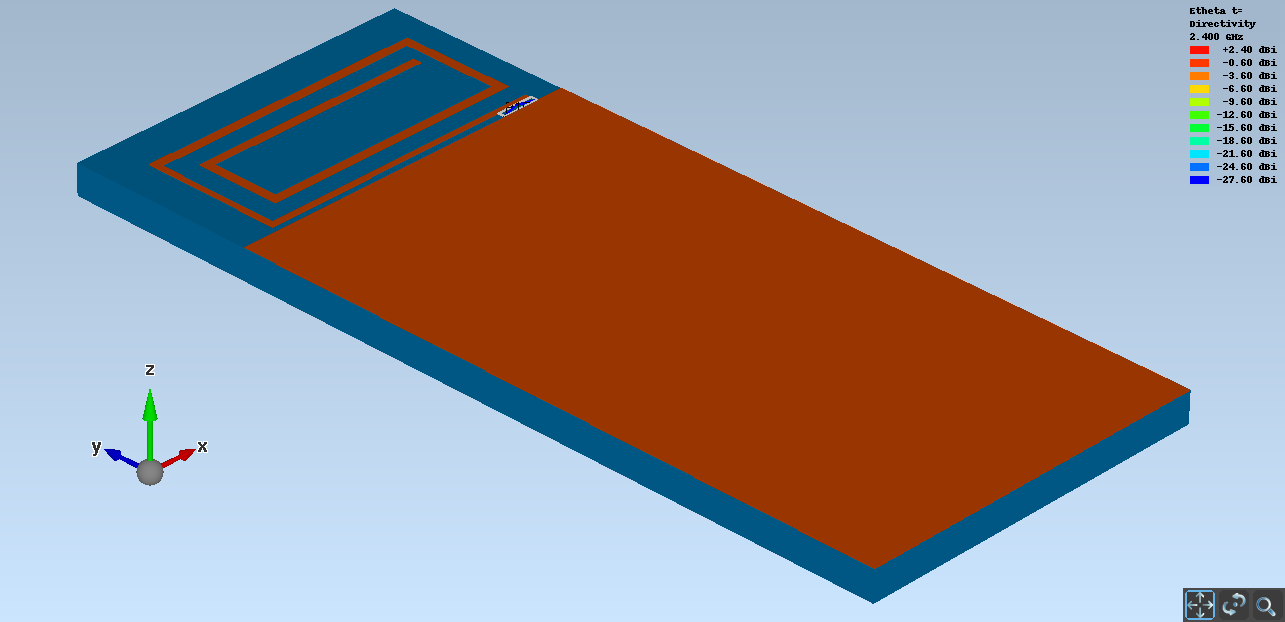
\includegraphics[width=0.75\textwidth]{../fig/plt/crazy_stuff_l2_3d_model.png}
	\caption{3D Modell}
\end{figure}



\clearpage
\subsubsection{Reflexionsfaktor $S_{11}$}
\begin{figure}[h!]
	\centering
	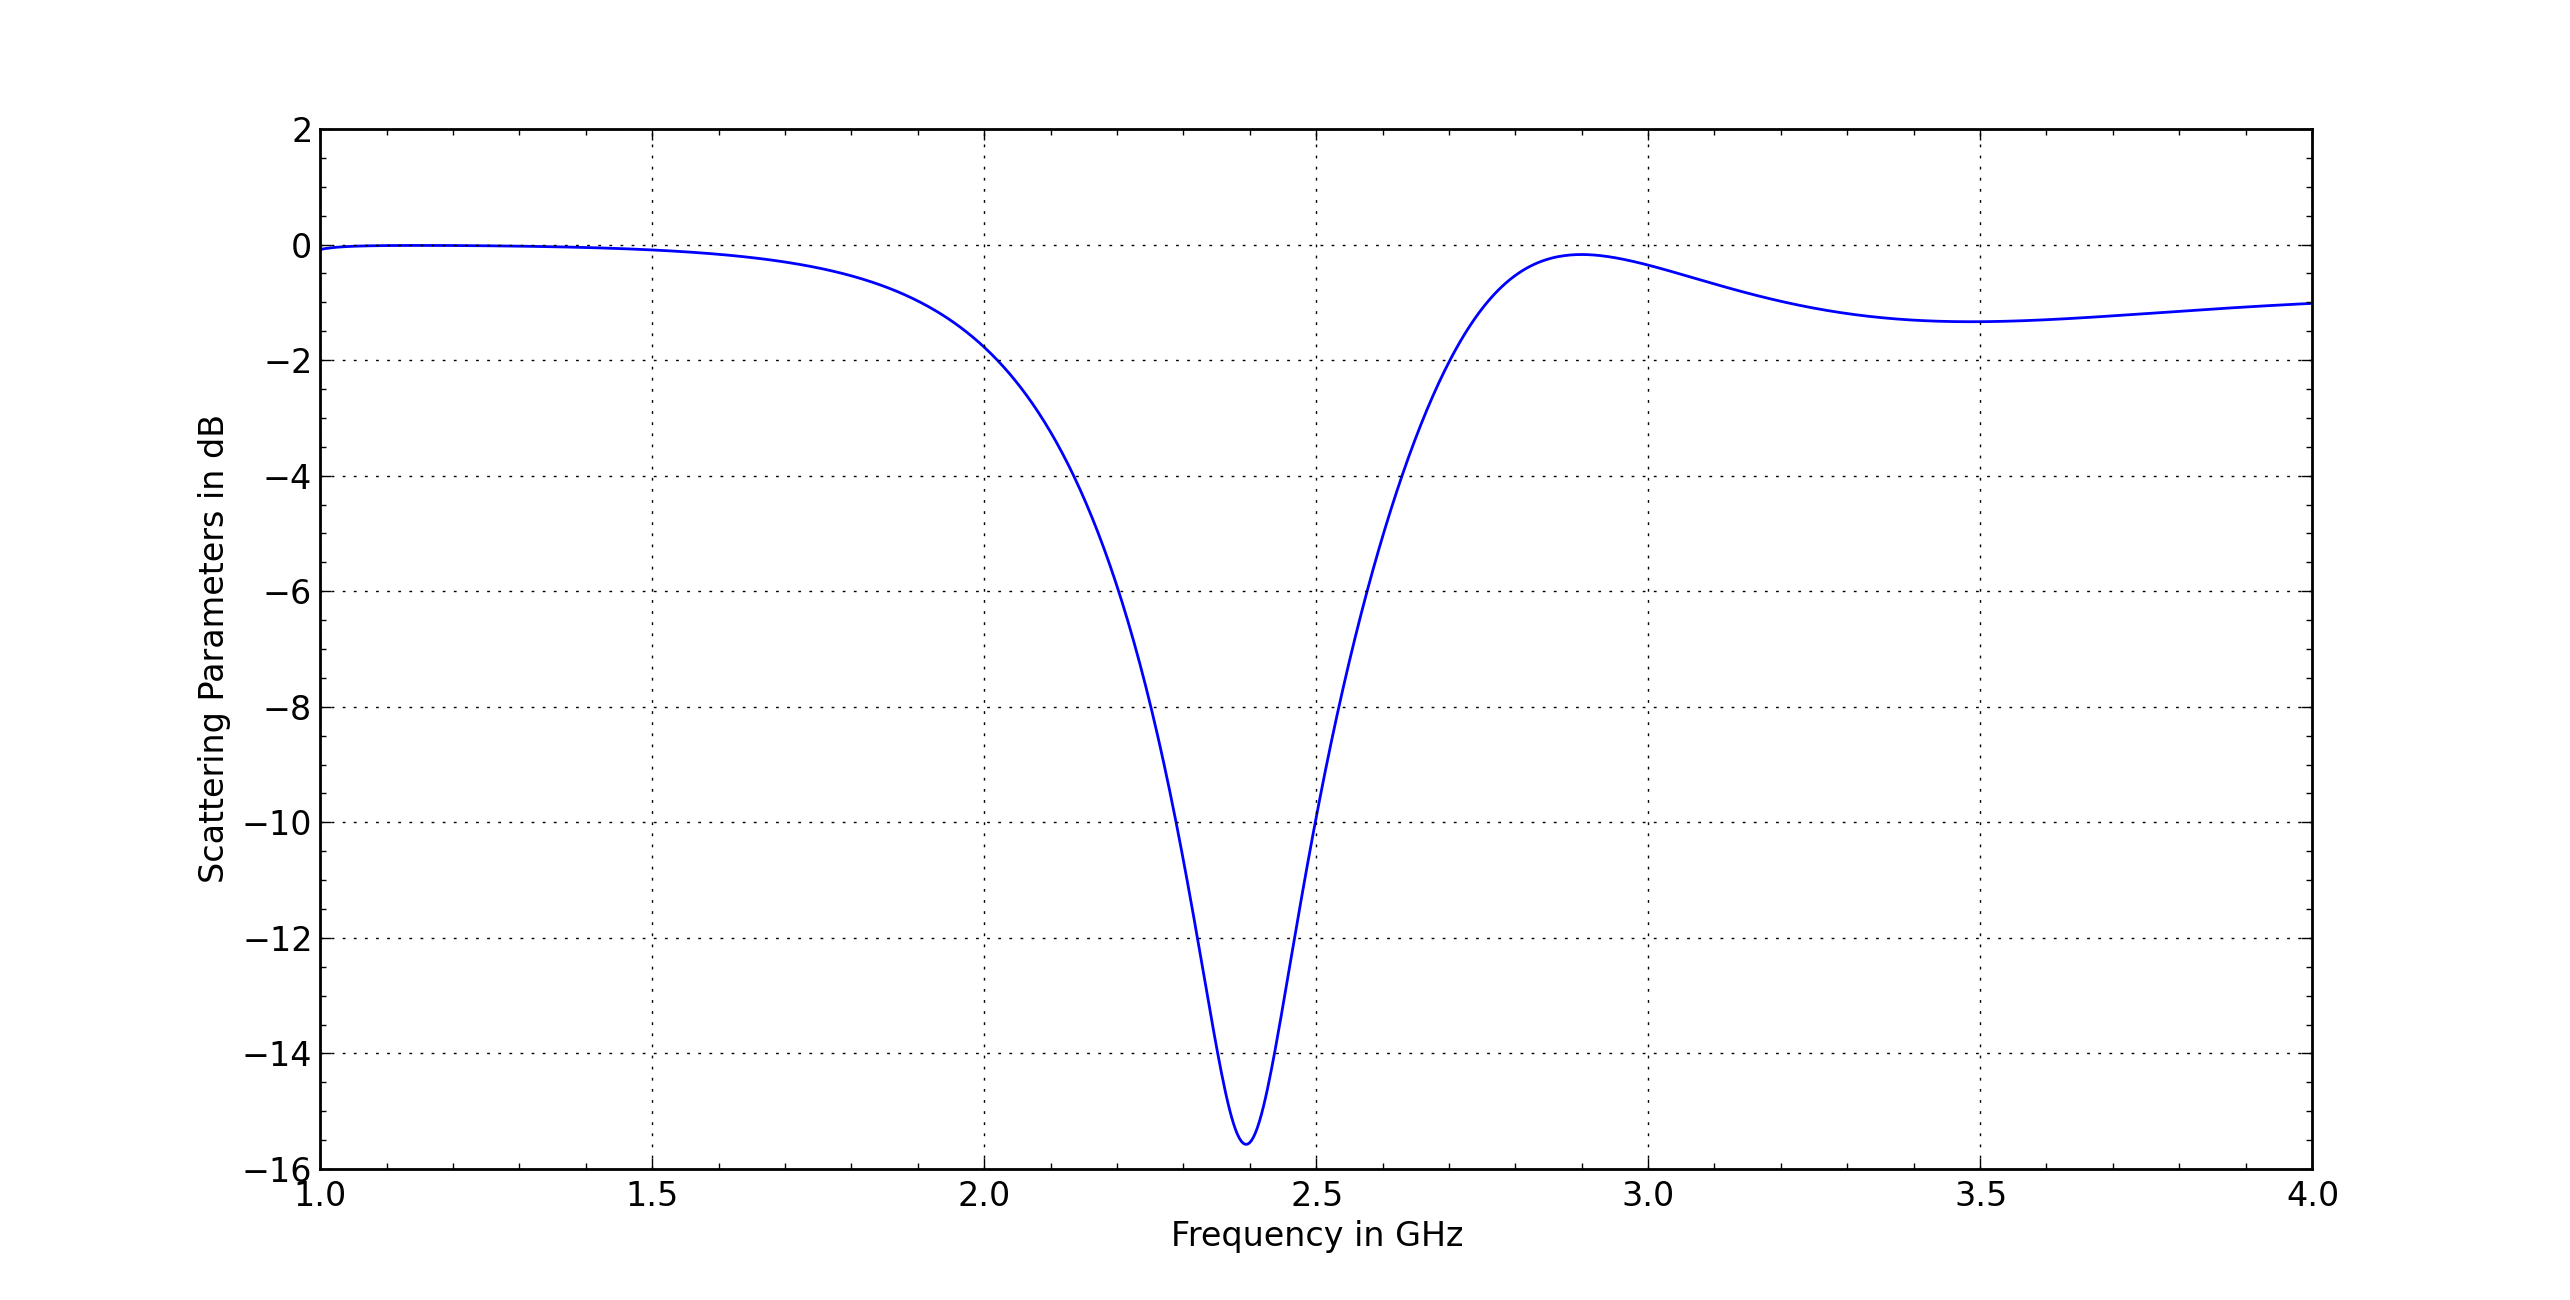
\includegraphics[width=0.8\textwidth]{../fig/plt/crazy_stuff_l2_s11.png}
	\caption{Reflexionsfaktor $S_{11}$}
\end{figure}

%\clearpage
\subsubsection{Impedanz}
\begin{figure}[h!]
	\centering
	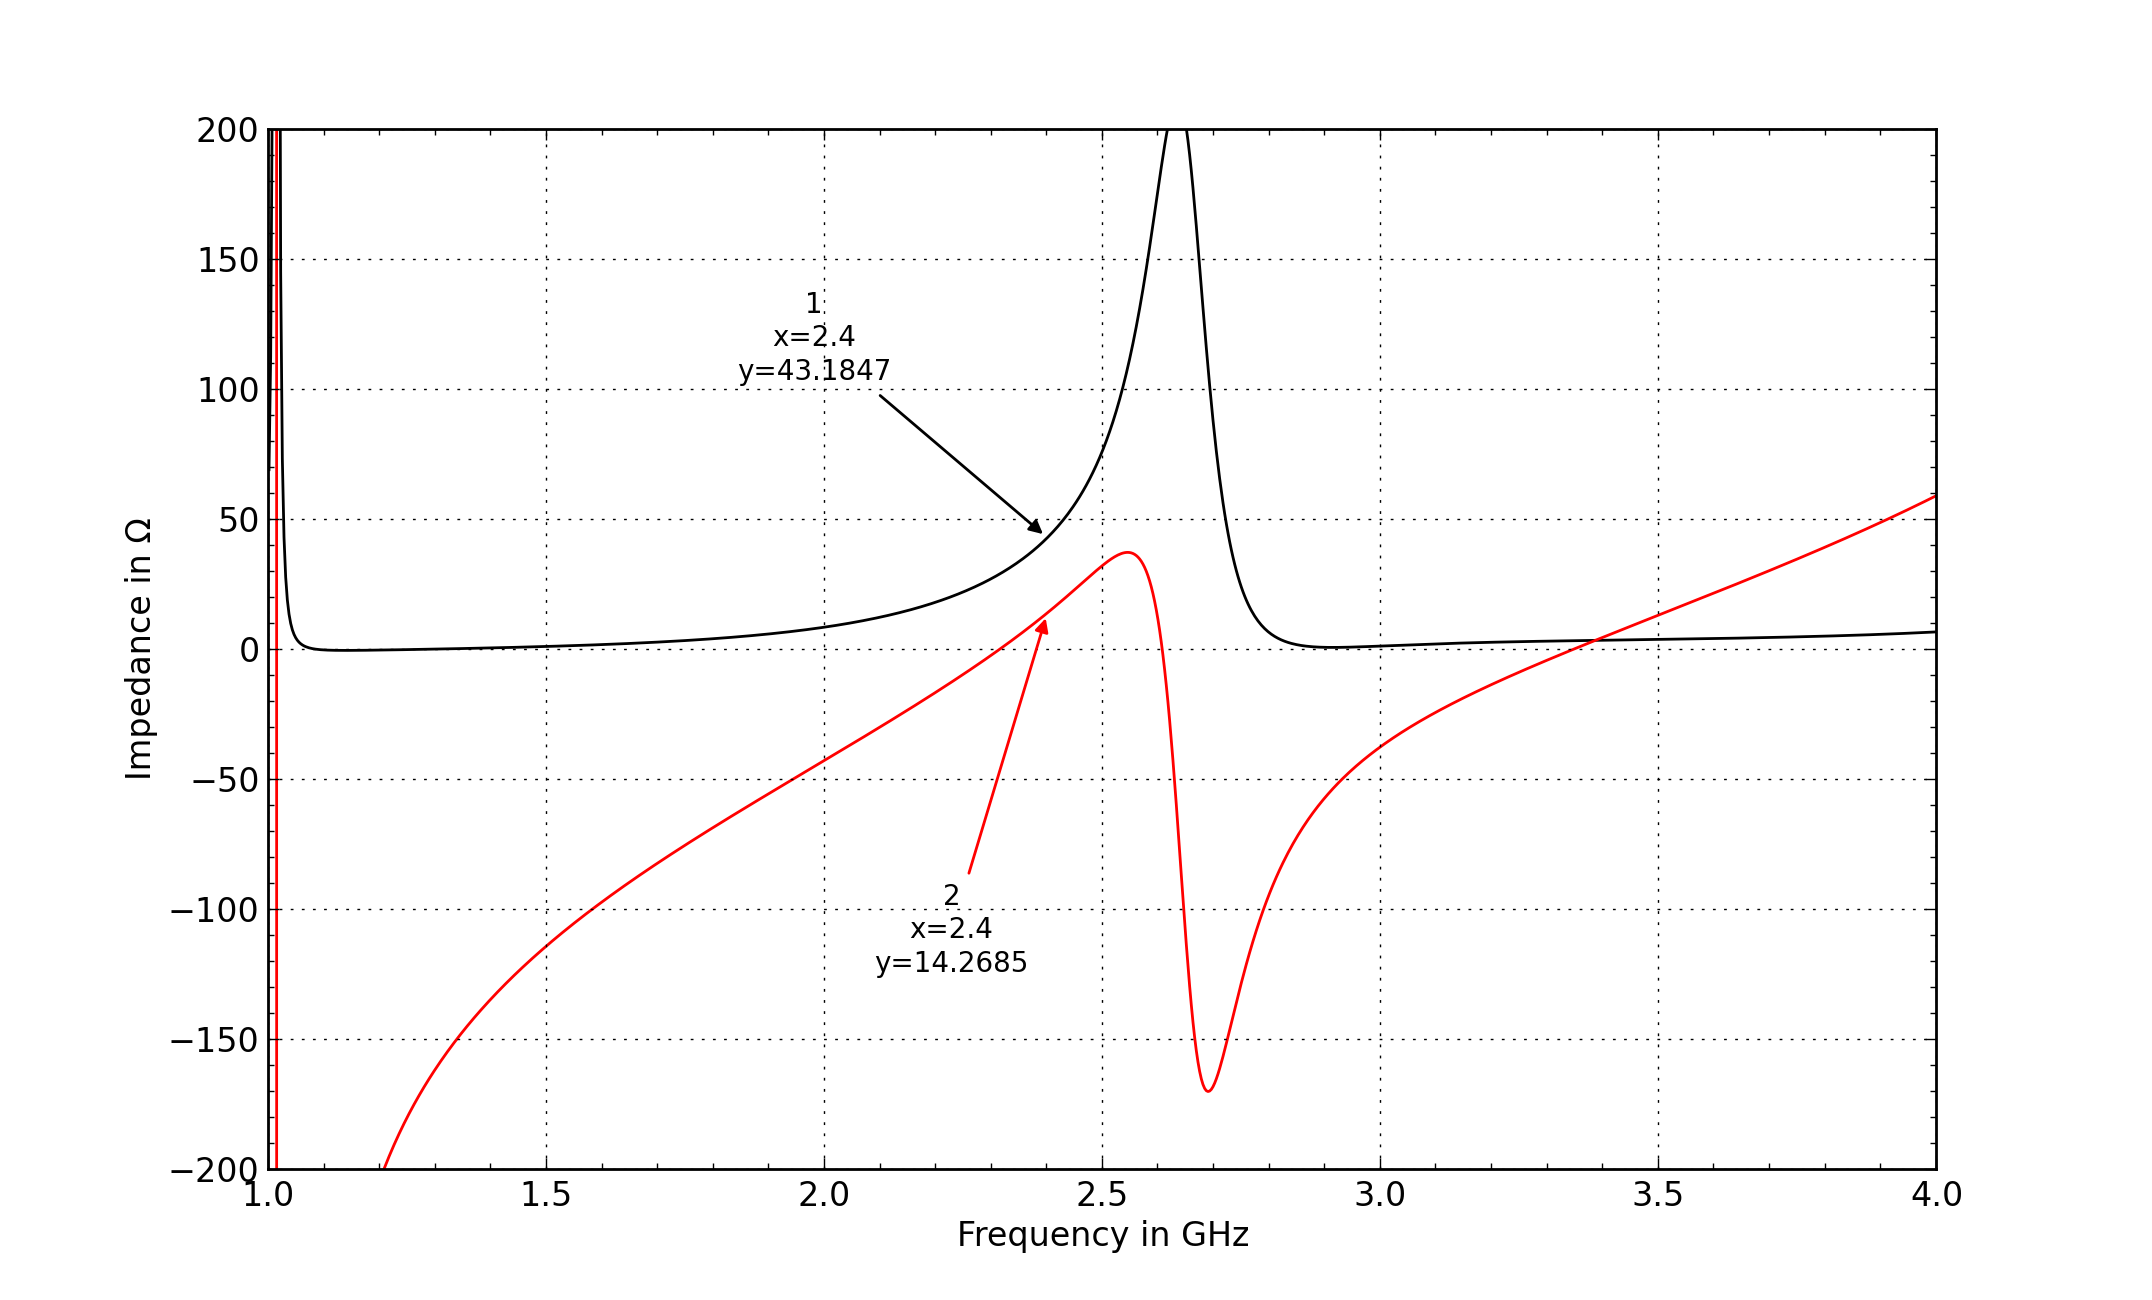
\includegraphics[width=0.8\textwidth]{../fig/plt/crazy_stuff_l2_z.png}
	\caption{Impedanz}
\end{figure}

\clearpage
\subsubsection{Fernfeld}
\begin{figure}[h!]
	\centering
	\begin{subfigure}[b]{0.96\textwidth}
		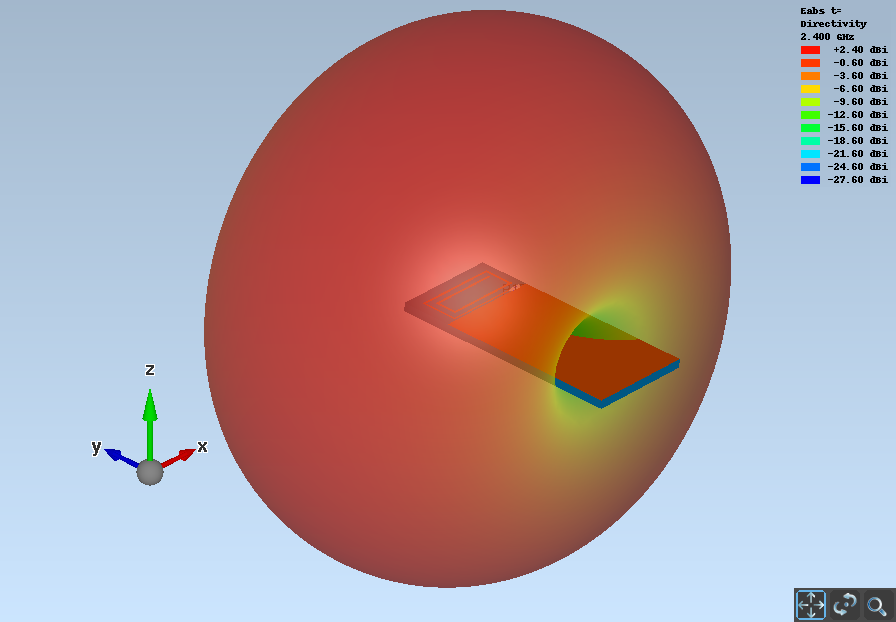
\includegraphics[width=1\textwidth]{../fig/plt/crazy_stuff_l2_3d_eabs.png}
		\caption{$\vec{E}_{\mathrm{abs}}$}
	\end{subfigure}

	\begin{subfigure}[b]{0.48\textwidth}
		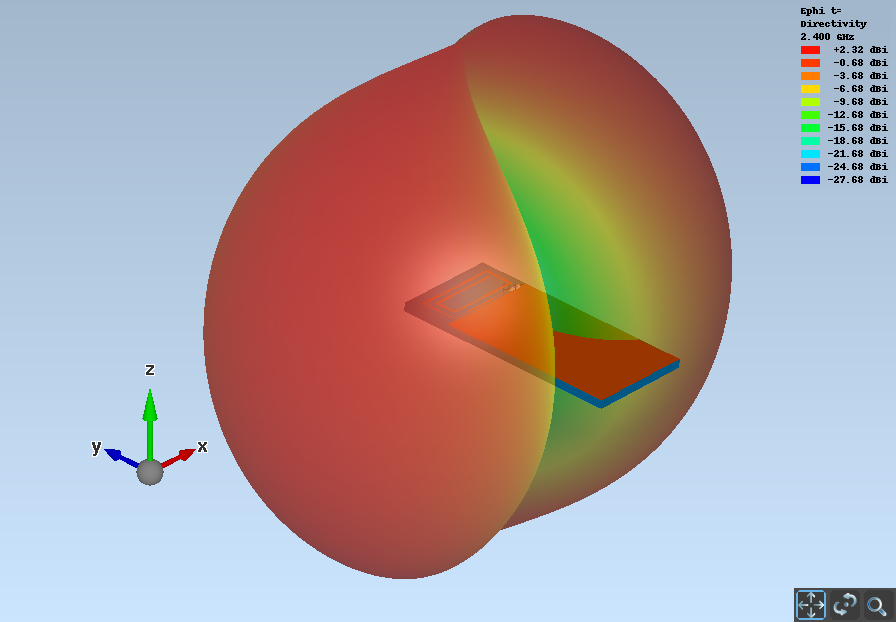
\includegraphics[width=1\textwidth]{../fig/plt/crazy_stuff_l2_3d_ephi.png}
		\caption{$\vec{E}_{\varphi}$}
	\end{subfigure}
	\begin{subfigure}[b]{0.48\textwidth}
		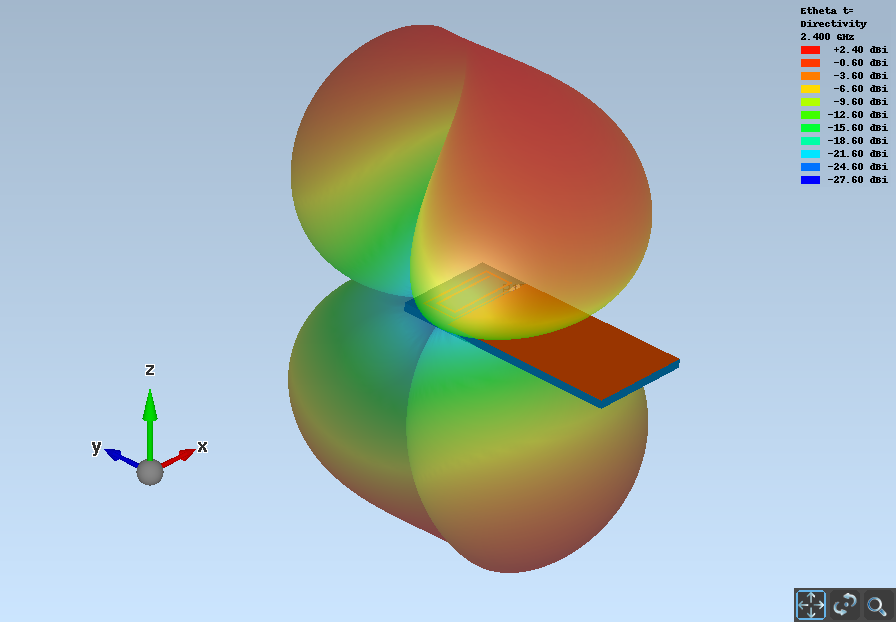
\includegraphics[width=1\textwidth]{../fig/plt/crazy_stuff_l2_3d_etheta.png}
		\caption{$\vec{E}_{\Theta}$}
	\end{subfigure}
	\caption{$\vec{E}$ Fernfeldanalyse (3D)}
\end{figure}


